\documentclass{article}

\bibliographystyle{alpha}
\usepackage{textcomp}
\usepackage{amsmath}
\usepackage{amssymb}
\usepackage{graphicx}
\usepackage{amsthm}
\newtheorem{thm}{Theorem}
\newtheorem{lem}{Lemma}

\author{Aditya Modi}
\title{A study of Splay Trees: Self adjusting binary search trees}
\date{\today}

\begin{document}
\maketitle
\section{Introduction}
Binary search trees are a fundamental data structure in computer science. A BST is a binary tree containing the items of the set, one item per node, with the items arranged in symmetric order. Generally, the information represented by each node is a record rather than a single data element. The major advantage of binary search trees over other data structures is that the related sorting algorithms and search algorithms such as in-order traversal can be very efficient. Basic operations supported in a BST are access, delete and insert and other comparison routines. These takes O(d)time, where d is the depth of the node containing the accessed item or the depth of the terminal leaf through which we leave our tree.\\
Most optimal BST's are all designed to reduce the worst-case time per operation. Sleator and Tarjan presented a paper (\cite{splay}) which restructured a BST on the view that in typical applications of search trees, not one but a sequence of operations is performed, and what matters is the total time the sequence takes, not the individual times of the operations. The splay tree, as developed by them, uses a simple restructuring heuristic called \emph{splaying} whenever a tree node is accessed. On an $n$-node splay tree, all the standard search tree operations have an amortized time bound of $O(log n)$ per operation, where by “amortized time” is meant the time per operation averaged over a worst-case sequence of operations. Thus splay trees are as efficient as balanced trees when total running time is the measure of interest.
\section{Intuition and Philosophy}
Balanced BST's maintain some constraint information at all times. For instance, \emph{color} of nodes is maintained in \emph{red-black trees} and \emph{heights} of nodes in \epmh{AVL-trees}. The basic idea is to be lazy and only restructure or rebalance the tree when required. The time difference from effecient searches is used in the search required for the ineffecient searches and restructuring time of the tree.\\
The intuition can be obtained from the fact that heavy children in any tree lead to imbalance in the structure in the tree thereby increasing the total time over a sequence of operations. We make these heavy children go away; we promote them and move an accessed node to the root of the tree in the restructuring. This differs from the move-to-root routine suggested by Allen and Munro \cite{alm}.
\section{Splaying}
In the splaying routine, the node accessed say $t$ is moved to the root of the tree using simple rotations. This reduces the depth of all nodes on the access path of $t$ to around half of their initial value. Some shallow nodes may although be pushed down by a depth of one or two. The rotations done depend on the nature of the access path.  To splay a tree at a node $x$, we repeat the following splaying step until $x$ is the root of the tree :
\begin{itemize}
\item zig:  If $p(x)$ , the parent of $x$, is the tree root, rotate the edge joining $x$ with $p(x)$. (This case is terminal).
\item zig-zig:  If $p(x)$ is not the root and $x$ and $p(x)$ are both left or both right children, rotate the edge joining $p(x)$ with its grandparent $g(x)$ and then rotate the edge joining $x$ with $p(x)$.
\item zig-zag:  If $p(x)$ is not the root and $x$ is a left child and $p(x)$ a right child, or vice-versa, rotate the edge joining $x$ with $p(x)$ and then rotate the edge joining $x$ with the new $p(x)$.
\end{itemize}
\begin{figure}[!htpb]
	\label{fig:rot}
	\begin{center}
		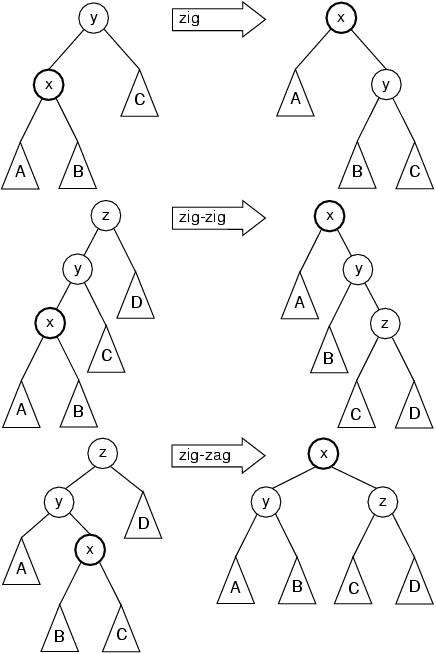
\includegraphics[width=0.4\columnwidth,height=0.6\columnwidth]{zigzag2.jpg}
	\end{center}
	\caption{Zig, zig-zig and zig-zag}
\end{figure}
Splaying at a node \emph{x} of depth \emph{d} takes \emph{O(d)} time, that is, time proportional to the time to access the item in \emph{x}. Splaying not only moves \emph{x} to the root, but roughly halves the depth of every node along the access path (See Fig. 2 and 3). This halving effect makes splaying efficient and is a property not shared by other, simpler heuristics, such as move to root. Producing this effect seems to require dealing with the zig-zig and zig-zag cases differently.
\begin{figure}[!htpb]
	\label{fig:splay}
	\begin{center}
		%\includegraphics[width=0.6\columnwidth,height=0.6\columnwidth,keepaspectratio]{splay.GIF}
		\includegraphics[width=0.7\columnwidth, height=0.7\columnwidth, keepaspectratio]{splay.GIF}
	\end{center}
	\caption{A splay operation on node A}
\end{figure}
\begin{figure}[!htpb]
	\label{fig:splay2}
	\begin{center}
		\includegraphics[width=0.5\columnwidth,height=0.5\columnwidth,keepaspectratio]{splay2.gif}
	\end{center}
	\caption{A splay operation on node B}
\end{figure}
\section{Analysis}
We shall analyze the amortized complexity of splaying through the potential method\footnote{Refer \cite{amort} for details on amortized analysis.} i.e.~by using a \emph{potential} function for analysis of amortized costs to carry out the amortization. In the potential method, a function $\phi$ is chosen that maps state of the data structure to non-negative numbers. If S is a state of the data structure, $\phi(S)$ may be thought of intuitively as an amount of potential energy stored in that state, alternatively, $\phi(S)$ may be thought of as representing the amount of disorder in state S or its distance from an ideal state. The amortized cost of a single operation say \emph{a} is then given by the relation:
\begin{align}
\label{eq:amc}
a = t+\phi ' - \phi
\end{align}
here, \emph{t} is the actual cost of the operation, $\phi '$ is the potential after the operation and $\phi$ is the potential before the operation. With this definition, we can estimate the total time of a sequence of \emph{m} operations by :
\begin{align}
\label{eq:tamc}
\sum_{j=1}^m t_j &=& \sum_{j=1}^m(a_j + \phi_{j-1} - \phi_{j}) &=& \sum_{j=1}^m a_j + \phi_0 - \phi_m
\end{align}
Now if we can obtain a bound on the amortized costs for the splaying routines employed and a bound for the decrease in potential, we can obtain an upper bound on the actual cost over a sequence of \emph{m} operations.
\subsection{Potential of a tree}
The potential of a splay tree, is defined by assuming that each item $i$ has a positive weight $w(x)$, whose value is arbitrary but fixed. The size $s(x)$ of a node $x$ in the tree is defined to be the sum of the individual weights of all items in the subtree rooted at $x$. Similarly, the rank $r(x)$ of node $x$ is taken to be $\log{s(x)}$. Finally, we define the potential of the tree to be the sum of the ranks of all its nodes.\\
Consider a sequence of $m$ accesses on an $n$-node splay tree. In analyzing the running time of such a sequence, it is useful to note that if the weights of all items remain fixed, then the net decrease in potential over the sequence is at most $\sum_{i=1}^n \log{W/w(i)}$ where $W=\sum_{i=1}^n w(i)$, since the size of the node containing item $i$ is at most $W$ and at least $w(i)$.
\subsection{Access Lemma}
As a measure of the running time of a splaying operation, the number of rotations done are used, unless there are no rotations, in which case one is charged for the splaying. Sleator and Tarjan used the following \emph{Lemma} for obtaining bounds on splaying routines.
\begin{lem}[Access Lemma]
\label{lem:acl}
The amortized time to splay a tree with root $t$ at a node $x$ is at most $3( r(t)- r(x))+ 1 = O(log(s(
 t)/s(x))$.
\end{lem}
Therefore, obtaining the above bounds on individual splaying operations and the potential change, we can get upper bound on the actual cost by eq.~\ref{eq:tamc}.
\section{Performance Theorems}
By using different weights of the nodes we can obtain bounds for different cases and compare them to other optimal binary search trees.
\begin{thm}[Balance Theorem]
\label{thm:bal}
The total access time for a sequence of $m$ accesses for a splay tree of size $n$ is 
\begin{align}
O((m + n)\log n + m)
\end{align}
\end{thm}
In other words, splay trees perform as well as static balanced binary search trees on sequences of at least $n$ accesses.
\begin{thm}[Static Optimality Theorem]
\label{thm:statop}
Let $q_i$ be the number of times element $i$ is accessed in sequence of accesses $S$. The cost of performing $S$ is 
\begin{align}
O(m+ \sum_{i=1}^n q_i log(m/q_i))
\end{align}
\end{thm}
In other words, splay trees perform as well as optimum static binary search trees on sequences of at least $n$ accesses.
\begin{thm}[Static Finger Theorem]
\label{thm:statfin}
Let $i_j$ be the element accessed in the $j^{th}$ access of $S$ and let $f$ be any fixed element (\emph{the finger}). The cost of performing $S$ is 
\begin{align}
O(m+ n\log n + \sum_{j=1}^m {\log |i_j - f| + 1})
\end{align}
\end{thm}
\begin{thm}[Working Set Theorem]
\label{thm:work}
Let $t(j)$ be the number of distinct elements accessed between access $j$ and the previous time element $i_j$ was accessed. The cost of performing $S$ is 
\begin{align}
O(m+ n\log n + \sum_{j=1}^m \log(t(j)+1))
\end{align}
\end{thm}
The above theorem states that we can bound the access time of an item $i$ by the logarithm of the number of different nodes we accesses sice its last access. Therefore, splay trees have a very nice property of very effecient access of recently accessed items.\\
Since the weights chosen for proving the above theorems are arbitrary, splay trees conform to these in every case. Therefore combining all the above we can bound the actual time by the least among all.
\section{Updation in splay trees}
Update operations can be done on binary search trees using splaying in two manners:
\begin{itemize}
\item By using $join(t_1,t_2)$ and $split(i,t)$ for the $delete(i,t)$ and $insert(i,t)$ routines.
\item Or by using the modified version of regular insert and update routines for a BST.
\end{itemize}
\subsection{Insert}
To insert a node $x$ into a splay tree:
\begin{itemize}
\item First insert the node as with a normal binary search tree.
\item Then splay the newly inserted node x to the top of the tree.
\end{itemize}
\begin{figure}[!htpb]
	\label{fig:splay2}
	\begin{center}
		\includegraphics[width=0.6\columnwidth,height=0.5\columnwidth,keepaspectratio]{img200.gif}
	\end{center}
	\caption{A delete operation}
\end{figure}
Alternately to carry out insert we firstly perform $split(i,t)$ and replace $t$ with $i$ as new root having the subtrees $t_1$ and $t_2$ returned by the split operation as its children.
\subsection{Deletion}
To delete a node $x$ from a splay tree:
\begin{itemize}
\item First delete the node as with a normal binary search tree.
\item Then splay the parent of the removed node to the top of the tree.
\end{itemize}
\begin{figure}[!htpb]
	\label{fig:splay2}
	\begin{center}
		\includegraphics[width=0.6\columnwidth,height=0.6\columnwidth,keepaspectratio]{img201.gif}
	\end{center}
	\caption{A delete operation}
\end{figure}
Alternately to carry out delete, we perform $access(i,t)$ and then replace $t$ by the join of its left and right subtrees.\\
The analysis of the updation operations show that they also follow the same efficient bounds as other search trees. Thus a new balance theorem can be suggested.
\begin{thm}[Balance Theorem with Updates]
\label{thm:upbal}
The total time for a sequence of $m$ arbitrary operations on a collection of initially empty splay trees having $n_j$ nodes in operation $j$ is 
\begin{align}
O(\sum_{j=1}^m \log n_j + m)
\end{align}
\end{thm}
\section{Variants \& other theorems}
The use of rotations in splay operations enables us to easily augment the data structure in the same way we can do for other search trees. But it uses heavy restructuring for providing effecient time bounds on standard operations. We can change our splaying routines and avoid redundant pointer assignments by performing \emph{top-down splaying} i.e.~perform inline rotations while going down the access path itself. Other ways suggested were semi-splaying and long-splaying. Refer to \cite{splay} for more on these.\\
An important result	was suggested by Wenger and later published by Tarjan (refer \cite{seq})which laid down the proof for following theorem:
\begin{thm}[Sequential Access theorem]
\label{thm:seq}
Accessing the n elements of a splay tree in symmetric order takes $O(n)$ time, regardless of the initial structure of the splay tree.\
\end{thm}
Apart from the above theorems, Tarjan and Sleator also suggested the following theorem of great value which still remains unproven:
\begin{thm}[Dynamic Optimality Conjecture]
\label{thm:doc}
Let $A$ be any binary search tree algorithm that accesses an element $x$ by traversing the path from the root to $x$ at a cost of $d(x)+1$, and that between accesses can make any rotations in the tree at a cost of 1 per rotation. If $A(S)$ is the cost for $A$ to perform the sequence $S$ of accesses. Then the cost for a splay tree to perform the same accesses is $O(n + A(S))$.
\end{thm}
\section{Conclusions}
We therefore see that splay trees give effecient performance by self optimisation. In this frequently accessed nodes are moved nearer to the root where they can be accessed more quickly. The worst case height is $O(n)$ but it doesn't matter if we are concerned over the time taken per operation for a sequence of sufficiently long operations as in that case it averages at $O(\log n)$.  Having frequently used nodes near the root is an advantage for nearly all practical applications and is particularly useful for implementing \emph{caches} and \emph{garbage collection} algorithms.
The advantages of splay trees over other search trees are:
\begin{itemize}
\item Simple implementation — simpler than other self-balancing binary search trees, such as \emph{red-black trees} or \emph{AVL trees}.
\item Comparable performance — average-case performance is as efficient as other trees.
\item More memory effecient — splay trees do not have to maintain any constraint data like other balanced search trees.
\item We can create a \emph{persistant data structure} version of splay trees which again requires $O(\log n)$ update.
\item No problem with equal keys and also maintains order between equal keys like stable sorting algorithms.
\end{itemize}
The disadvantages of splay trees may be:
\begin{itemize}
\item Splay trees cannot be used in real-time applications, where optimal performance for each query is desired.
\item The tree is resructured after every access operation, which may prove to be bad if same structure has to be maintained for future operations.
\item A lot of restructuring is done which may not be a desired trait.
\end{itemize}
The following applications of splay trees are prominent:
\begin{itemize}
\item Cache impletation
\item Data compression
\item Encryption
\item Implementation of link-cut trees and Euler trees
\item Merging and splitting of trees.
\end{itemize}
The simple and evolving nature of splay trees and its restructuring heuristic proves to be very useful and are at least as effecient as any corresponding balanced data structure.
\bibliography{ref}
\end{document}